\newcommand\hilight[2]{\color{#1}#2\color{black}}
\definecolor{grey}{RGB}{127,127,127}
\definecolor{darkcyan}{RGB}{0,127,127}
\definecolor{olivegreen}{RGB}{0,127,0}
\definecolor{violet}{RGB}{127,0,127}
\definecolor{brickred}{RGB}{127,0,0}
\definecolor{brown}{RGB}{127,63,0}
\definecolor{red}{RGB}{127,0,0}

\section{Landslide}
\label{sec:landslide}

Landslide is based on the technique of systematic exploration~\cite{verisoft}, a way of exploring the state space of different possible thread interleavings in a concurrent system.
It follows in the footsteps of related tools such as CHESS~\cite{chess}, dBug~\cite{dbug-ssv}, and DeMeter~\cite{demeter}, but is the first tool we know of to apply systematic exploration in a kernel environment.
In this section we give an overview of Landslide's design and interface, and point out the annotations students need to provide to make Landslide work with their own code.

%%%%%%%%%%%%%%%%%%%%%%%%%%%%%%%%%%%%%%%%%%%%%%%%%%%%%%%%%%%%%%%%%%%%%%%%%%%%%%%%
\subsection{Scope}

\paragraph{Testing environment}
Landslide is implemented as a module for Simics, the simulator our students use as an execution environment for their kernels. Simics can load Landslide while booting a kernel, and calls into Landslide once per instruction and once per memory access of the simulated execution.
Landslide uses this information to update its internal representation of the kernel's state, which it in turn uses to decide how to control the kernel's execution.

\paragraph{Limitations}
Landslide assumes that timer interrupts are the only nondeterministic events that influence a kernel's concurrent execution. While this prevents us from finding races related to external input such as disk or network I/O, Landslide is already able to find many types of complicated races by controlling timer-driven thread scheduling.
Landslide's model is also restricted to uniprocessor execution.
Supporting multiprocessor environments and device driver testing is left to future work.
% this used to say ", and production kernels"

% TODO: This paragraph can be removed if we're hurting for space
We also note that, in contrast with stress testing, Landslide works best with very small test cases. While a more conventional stress test achieves coverage by exercising many system calls (in parallel and/or in sequence), Landslide's coverage results from exploring the different scheduling possibilities that arise from a short sequence of system calls.
If Landslide were used when running a stress test, the resulting state space would be too large to explore feasibly.
Hence, when working with students, we provided a suite of four test programs, each no longer than 10 lines of code.

%%%%%%%%%%%%%%%%%%%%%%%%%%%%%%%%%%%%%%%%%%%%%%%%%%%%%%%%%%%%%%%%%%%%%%%%%%%%%%%%
\subsection{Example}
% TODO: if necessary, this can be not its own section

Figure~\ref{fig:threadfork} shows a timer-dependent bug common in many Pebbles implementations which we will use as a running example in the rest of this section. This code is a simplified implementation of the \x{thread_fork} system call: it constructs data structures necessary for the new thread, then asks the scheduler to make the new thread runnable, then returns its assigned thread ID. However, if the timer preempts execution at line~\ref{line:hax}, the child thread might run and invoke \x{exit}, causing \x{child} to become a dangling pointer.

\begin{figure}[t]
\small
\begin{lstlisting}[numbers=left]
int thread_fork() {
	thread_t *child = construct_new_thread();
	add_to_runqueue(child);
	// at this point child may run and exit#\label{line:hax}#
	return child->tid;#\label{line:owned}#
}
\end{lstlisting}
\caption{Example race condition. If a timer interrupt occurs at line~\ref{line:hax}, the child thread can run, exit, and free its state, causing line~\ref{line:owned}'s access to be a use-after-free.}
\label{fig:threadfork}
\end{figure}

%%%%%%%%%%%%%%%%%%%%%%%%%%%%%%%%%%%%%%%%%%%%%%%%%%%%%%%%%%%%%%%%%%%%%%%%%%%%%%%%
\subsection{Testing Mechanism}

Systematic exploration, Landslide's mechanism for testing different concurrent scenarios, uses the idea of an {\em execution tree} to enumerate all possible thread interleavings in a system. These interleavings are defined around {\em decision points}, which intuitively indicate points during execution at which a preemption could cause different behaviour to arise.
Searching with few decision points results in coarser-grained interleavings, shorter test execution, and less likelihood of finding bugs; searching with more results in the opposite.

Landslide ``explores'' decision trees by controlling the kernel's execution in two ways.
First, at each decision point, it can force an arbitary thread to run in place of the current one by injecting timer interrupts to force the kernel to context switch.
Second, whenever the kernel finishes executing a particular interleaving of the test case, it reverts the system to an earlier state to explore additional interleavings using Simics's backtracking mechanism.

In our example bug, the necessary decision point for finding the bug is at line~\ref{line:hax}. With correct annotations (discussed in Section~\ref{sec:instrument} and shown in Figure~\ref{fig:annotation}), Landslide can automatically identify this decision point.
Landslide also automatically identifies a minimal set of decision points at voluntary reschedules between threads (e.g. \x{yield}). Together these decision points define an execution tree which exposes the bug, depicted in Figure~\ref{fig:tree}.

Of course, additional decision points are necessary to expose more subtle race conditions. We provide an interface for adding new decision points to refine the state space, described in Section~\ref{sec:decision}.
In order to cope with the exponentially-sized nature of state spaces with many decision points, Landslide uses the Dynamic Partial Order Reduction (DPOR) algorithm~\cite{dpor} to identify and prune redundant thread interleavings, the specifics of which are beyond the educational scope of this work.
We also provide an interface for helping Landslide further reduce the state space by considering decision points only from certain components of the kernel, which we discuss in Section~\ref{sec:focusing}.

\begin{figure}[t]
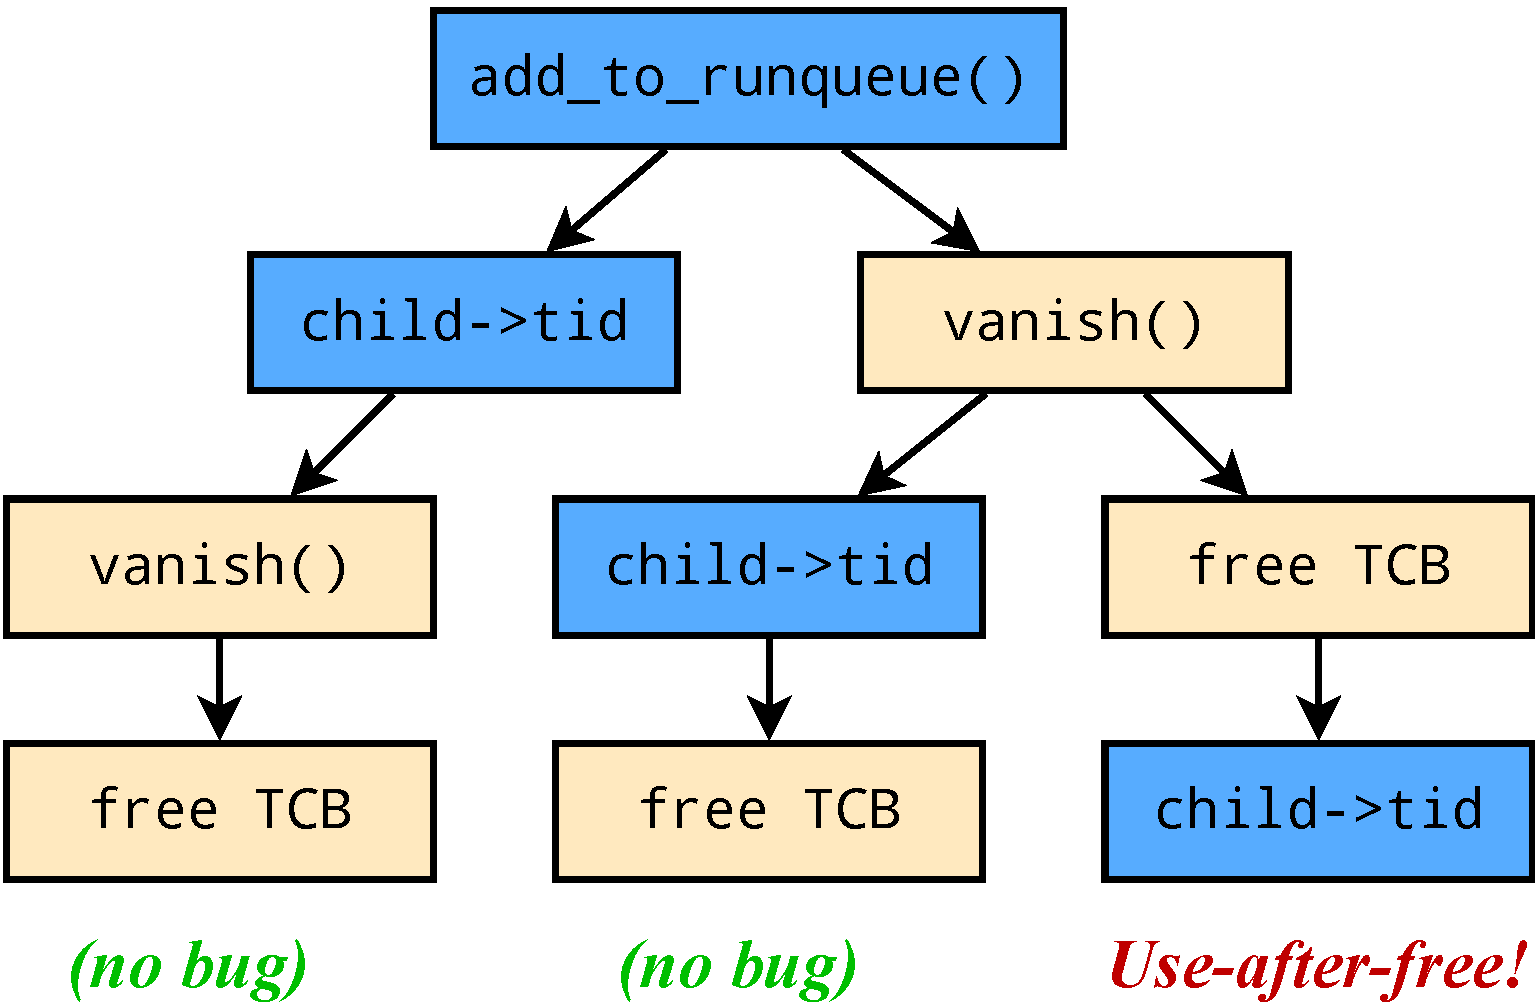
\includegraphics[width=0.48\textwidth]{threadfork/threadfork.pdf}
\caption{The state space of possible thread interleavings can be viewed as an {\em execution tree}.
Landslide uses timer interrupts to force different threads to run as it explores this tree.
If a kernel has concurrency errors, they will show up in some branches, but not others.
This tree shows the bug from Figure~\ref{fig:threadfork}, with decision points from the parent thread shaded.
}
\label{fig:tree}
\end{figure}

%%%%%%%%%%%%%%%%%%%%%%%%%%%%%%%%%%%%%%%%%%%%%%%%%%%%%%%%%%%%%%%%%%%%%%%%%%%%%%%%
\subsection{Identifying Bugs}

Landslide has several checks that detect when a bug arises. It can identify kernel panics, use-after-free accesses (and other memory errors such as double-free and memory leaks), and deadlocks.

Landslide can optionally also check heuristically for infinite loops and livelock. This is done by comparing the length of the current interleaving against previously-explored ones: if the current interleaving has been running disproportionately longer (by a large arbitrary constant factor), it indicates the kernel is likely stuck.
We have never found this technique to erroneously report false positives, although it may fail to trigger when it ought to if too few previous interleavings have been tested to make a reliable comparison.

When Landslide identifies a bug, it outputs a {\em decision trace}, an example of which is shown in Figure~\ref{fig:trace}.
This trace reports what kind of bug was detected (for uses-after-free, it also prints stack traces for when the block was allocated and freed), and also reports each decision point in the current interleaving: which thread was running, a trace of its stack when it was switched away from, and the thread that we caused to preempt it. With this trace, the student can better understand the concurrent execution that led to the bug.

In general, with false-negative bug detection, the kernel might execute a buggy behaviour yet Landslide would miss it. However (except in the case of heuristic infinite loop detection), when Landslide does identify a bug, the student can be sure that a race exists.

\newcommand\bug[1]{\hilight{red}{#1}}
\newcommand\decision[1]{\bfseries \hilight{olivegreen}{#1}}
\newcommand\stacktrace[1]{\hilight{darkcyan}{#1}}
\begin{figure}[t]
\begin{lstlisting}
#\bfseries \bug{USE~AFTER~FREE:~read~from~0x15a8f0~at~IP~0x104209}#
#\bug{Block~0x15a8f0~was~allocated~by~thread~3~at~(...)}#
                   #\bug{and~freed~by~thread~4~at~(...)}#
Decision trace follows:
#\decision{1:  switched from thread 3 -> thread 4 at:}#
        0x105a10 in #\stacktrace{context\_switch}#,
        0x1041f4 in #\stacktrace{thread\_fork}#,
        0x10362b in #\stacktrace{thread\_fork\_wrapper}#
#\decision{2:  switched from thread 4 -> thread 3 at:}#
        0x105a10 in #\stacktrace{context\_switch}#,
        0x104681 in #\stacktrace{yield}#,
        0x104570 in #\stacktrace{exit}#,
        0x103708 in #\stacktrace{exit\_wrapper}#
#\decision{Current thread 3 at:}#
        0x104209 in #\stacktrace{thread\_fork}#,
        0x10362b in #\stacktrace{thread\_fork\_wrapper}#
Total decision points 24, total backtracks 5
\end{lstlisting}
\caption{Landslide outputs this trace for Figure~\ref{fig:threadfork}'s bug.}
\label{fig:trace}
\end{figure}

%%%%%%%%%%%%%%%%%%%%%%%%%%%%%%%%%%%%%%%%%%%%%%%%%%%%%%%%%%%%%%%%%%%%%%%%%%%%%%%%
\subsection{Instrumentation}
\label{sec:instrument}

Landslide's interface is comprised of two types of instrumentation which students must provide: {\em required annotations} and {\em configuring decision points}.

\subsubsection{Required annotations}
Users annotate their kernels to inform Landslide of certain important concurrency events during execution. We provide a set of annotation functions, called \x{tell_landslide}, for this purpose. The annotations denote when a thread runs \x{fork}, \x{sleep}, or \x{exit}, when a thread is added to or removed from the runqueue, and when threads become blocked on mutexes.
Figure~\ref{fig:annotation} shows the code from Figure~\ref{fig:threadfork} with \x{tell_landslide} annotations.

There is also a configuration file, \x{config.landslide}, in which the user must specify constant information such as the function names of the timer handler and context switcher, which threads exist when the kernel boots, and which userspace test program Landslide should invoke.
Finally, there are two short (nominally two-line) functions used within Landslide itself that the user must implement. These are predicates on the kernel's scheduler state, and express potentially nontrivial conditions: whether the current thread is runnable but not on the runqueue, and whether preemption is disabled while interrupts are on.

\newcommand\telllandslide[1]{\bfseries \color{violet}{#1}}
\begin{figure}[t]
\small
\begin{lstlisting}
void add_to_runqueue(thread_t *child) {
	#\telllandslide{tell\_landslide\_thread\_runnable(child->tid);}#
	// ...
}
int thread_fork() {
	thread_t *child = construct_new_thread();
	#\telllandslide{tell\_landslide\_forking(child->tid);}#
	add_to_runqueue(child);
	return child->tid;
}
\end{lstlisting}
\caption{Landslide requires the programmer to annotate important concurrency events in their kernel. \texttt{tell\_landslide\_thread\_runnable()} indicates that a thread can henceforth be forced to run with timer interrupts, and \texttt{tell\_landslide\_forking()} announces a new thread's existence.}
\label{fig:annotation}
\end{figure}

\subsubsection{Configuring decision points}
\label{sec:decision}

Using only the decision points automatically identified on voluntary reschedules will result in coarse-grained interleavings likely to overlook bugs.
We provide an extra annotation
for the user to add more decision points for a finer-grained search, called
\x{tell_landslide_decide()}.
We recommend using it in concurrency primitives, such as at the start of \x{mutex_lock()} and at the end of \x{mutex_unlock()}.

\subsubsection{Focusing the search space}
\label{sec:focusing}

The strategy we described above may cause Landslide to identify decision points in unrelated parts of the kernel, such as when accessing mutexes in unrelated system calls.
We provide interface options in \x{config.landslide} for the student to view currently identified decision points and to selectively limit them.
First, the student writes ``\x{DECISION_INFO_ONLY}'' to make Landslide run only one interleaving and then print all decision points instead of continuing to explore.
Then, they write ``\x{within_function} \x{foo}'' to whitelist function \x{foo}, and ``\x{without_function} \x{bar}'' to blacklist function \x{bar}.
For example, if testing thread death and reaping, the student should write \x{within_function exit} and \x{within_function} \x{wait}, and also
(assuming they don't care about the virtual memory operations associated with \x{exit})
\x{without_function} \x{destroy_address_space}.

% Additionally, the student may configure Landslide's state space reduction to ignore certain memory locations.
% DPOR's analysis requires a memory independence relation between thread transitions; the more transitions are independent from each other, the more reduction can be achieved.
% Unfortunately, in the kernel environment, every thread switch will execute through a common path that modifies shared scheduler data structures.
% Unchecked, this would cause every transition to conflict with each other and result in no reduction in execution time from DPOR.
% Certain other shared memory conflicts also arise that are irrelevant to whichever system calls are being tested; for example, if testing for races in thread lifecycle routines, the user likely does not care about accesses to the frame allocator mutex.
%
% We provide an interface with which the user can configure Landslide to ignore such unrelated conflicts to more efficiently test components of the kernel they care about.
% In \x{config.landslide}, the user writes ``\x{ignore_sym}'' followed by the name of the global variable to ignore and its type size, and Landslide may then identify transitions as independent even if they conflict on that memory.

%%%%%%%%%%%%%%%%%%%%%%%%%%%%%%%%%%%%%%%%%%%%%%%%%%%%%%%%%%%%%%%%%%%%%%%%%%%%%%%%
\subsection{Evaluation}

We evaluated Landslide in two ways: first, by instrumenting two kernels we were familiar with to measure time spent to find different races, and second, by meeting with students of 15-410 in the Spring 2012 semester, before they submitted their kernel for grading, to see if they could find bugs on their own with Landslide.

We instrumented one kernel written by an author in a previous year, and also one kernel the same author manually graded as a teaching assistant.
We configured Landslide to search for five complicated already-known race conditions.
In addition to finding all five races, Landslide also found a sixth previously unknown race in said author's own kernel.
Using decision points only on calls to \x{mutex_lock} and on voluntary reschedules, Landslide found each of the six bugs in 11 to 57 seconds, executing between 1 and 377 distinct interleavings for each.

In the user study of current students, we found that students spent on average 119 minutes (60 to 158) on the required instrumentation, and a further 36 minutes (10 to 60) refining Landslide's search.
Of the four groups who finished the required part, all four found previously unknown bugs with Landslide: two races and two deterministic errors.
These bugs manifested as infinite loops, a kernel panic, and a use-after-free.

% TODO: decide whether to put table 7.2 from the thesis here. i think probably not?

